\subsection{Architecture générale}
	\begin{frame}
		\frametitle{Architecture générale}
		\begin{figure}
			\centering
			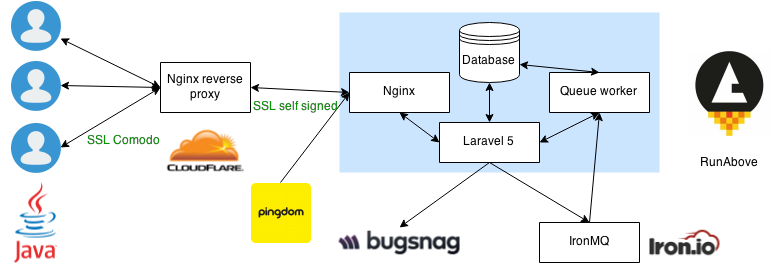
\includegraphics[width=1\textwidth]{images/architecture.png}
			\caption{Architecture générale}
			\label{fig:architecture-generale}
		\end{figure}
	\end{frame}

\subsection{Serveur}
	\begin{frame}
		\frametitle{API REST}
		\begin{itemize}
			\item Une API respectant les bonnes pratiques REST et HTTP;
			\item Entièrement en JSON;
			\item Une documentation claire et complète (\url{https://developers.diplo-lejeu.fr});
			\item Organisation en trois ressources : Conversations, Ordres, Parties;
			\item Documentation écrite en Markdown puis affichée sur une interface web.
		\end{itemize}
	\end{frame}

	\begin{frame}
		\frametitle{Composants}
		\begin{itemize}
			\item Framework MVC PHP : Laravel 5;
			\item ORM : Eloquent, intégré à Laravel;
			\item Base de données relationnelle : SQLite;
			\item Push / Pull Queue : IronMQ via \texttt{iron.io};
			\item Agrégateur d'exceptions : Bugsnag.
		\end{itemize}\bigskip
		Le tout hébergé sur un VPS chez RunAbove, à Roubaix. DNS et certificats SSL gérés par CloudFlare
	\end{frame}

	\begin{frame}
		\frametitle{Patterns utilisés}
		\begin{itemize}
			\item \textit{Repository pattern} : abstraction de l'accès au stockage;
			\item \textit{Middleware pattern} : pour les requêtes HTTP entrantes et la gestion des exceptions;
			\item \textit{Dependency injection} : injection automatique de classes concrètes implémentant des interfaces;
			\item Conception SOLID : beaucoup de classes spécialisées, contrôleurs HTTP de moins de 10 lignes.
		\end{itemize}
	\end{frame}

\subsection{Client}
	\begin{frame}
		\frametitle{Client}
	\end{frame}
